\documentclass[]{scrartcl}
\usepackage[utf8]{inputenc}
\usepackage{graphicx}
\usepackage{amsmath}
\usepackage{float}
\usepackage[ngerman, english]{babel} 
\usepackage{hyperref}
\hypersetup{
	colorlinks,
	citecolor=black,
	filecolor=black,
	linkcolor=black,
	urlcolor=black,
}
\selectlanguage{ngerman}

\title{Modellierung dynamischer Systeme  \\ Abgabe der Praktikumsaufgabe 1}

\author{Maria Lüdemann und Birger Kamp}

\begin{document}

\maketitle
\selectlanguage{ngerman}
\tableofcontents

\section{Teilaufgabe 1 - Steife Differentialgleichungen}
Es ist folgende DGL gegeben:\\
$ y' = 10 - 500y + 5000x $,
$ y(0) = 1 $\\
\\
Dazu ist folgende analytische Lösung gegeben:\\
$ y = 10x + e^{-500x}$ \\
\\
Für diese DGL ist ein Schaltbild in Simulink zu entwerfen. Des weiteren sollen die Verfahren(Runge-Kutta 2. Ordnung, expliziter Euler, impliziter Euler) erarbeitet und Iterationsgleichungen für die jeweiligen Verfahren angegeben werden. Im Anschluss soll ein Programm entwickelt(\textit{stiff}) werden das das jedes Verfahren auf die DGL anwendet und in einem Plot zum Vergleich mit der gegebenen analytischen Lösung anzeigt. Zum weiteren Vergleich soll ein Plot berechnet werden der die Differenz zwischen den Verfahrenslösungen und der analytischen Lösung darlegt.\\
Das Programm (\textit{stiff}) soll mit vier Parameter Varianten gestartet werden, die sich wie folgt beschreiben:
\begin{itemize}
	\item $h = 0.001,  x_{End} = 0.2 $
	\item $h = 0.003,  x_{End} = 0.2 $
	\item $h = 0.004,  x_{End} = 0.2 $
	\item $h = 0.005,  x_{End} = 0.2 $
\end{itemize}

\subsection*{Schaltbild}
Das Simulink-Schaltbild zu dieser Gleichung ist:

\begin{figure}[H]
\centering
\includegraphics[width=1\linewidth]{a1_1_Schaltbild}
\caption{Simulink Schaltbild DGL1}
\label{fig:A1_1_Schaltbild}
\end{figure}

\subsection{Iterationsgleichungen}
Im Folgenden die Iterationsgleichungen der jeweiligen Verfahren.

\subsubsection{Explizites Euler-Verfahren}
\begin{align}
x_{n+1} = x_{n}+h \\
y_{n+1} = y_{n}+h*f(x_{n},y_{n}) \\
y_{n+1} = y_{n}+h*(10-500y_{n}+5000x_{n})
\end{align}

\subsubsection{Implizites Euler-Verfahren}
Das implizite Euler entspricht dem expliziten mit dem Unterschied das hier anstelle des $y_{n}$ ein $y_{n+1}$ genutzt wird, dass mithilfe geeigneter Verfahren zur Nullstellenberechnung approximiert werden muss. 
\begin{align}
x_{n+1} = x_{n}+h \\
y_{n+1} = y_{n}+h*f(x_{n+1},y_{n+1}) \\
y_{n+1} = y_{n}+h*(10-500y_{n+1}+5000x_{n+1})
\end{align}

\subsubsection{Runge-Kutta-Verfahren 2.Ordnung}
\begin{align}
x_{n+1} = x_{n}+h \\
k_{1} = h*f(x_{n},y_{n}) \\
k_{1} = h*(10-500y_{n}+5000x_{n}) \\
k_{2} = h*f(x_{n} + \dfrac{h}{2},y_{n} + \dfrac{k_{1}}{2}) \\
k_{2} = h*(10-500*(y_{n} + \dfrac{k_{1}}{2})+5000*(x_{n} + \dfrac{h}{2})) \\
y_{n+1} = y_{n}+k_{2}
\end{align}

\subsection{Plot der Lösungen}
Im Folgenden sind alle Plots der Ergebnisse der Verfahren dargestellt. Es wird außerdem jeweils die Ergebnis-Differenz eines Verfahrens zur analytischen Lösung gezeigt.
\subsubsection{h=0.001}
Das Ergebnis zeigt, dass die Verfahren bis x=0.01 sehr ähnliche Ergebnisse liefern und haben eine max. Differenz von ca. 0.12. Danach laufen alle Kurven kongruent.
\begin{figure}[H]
\centering
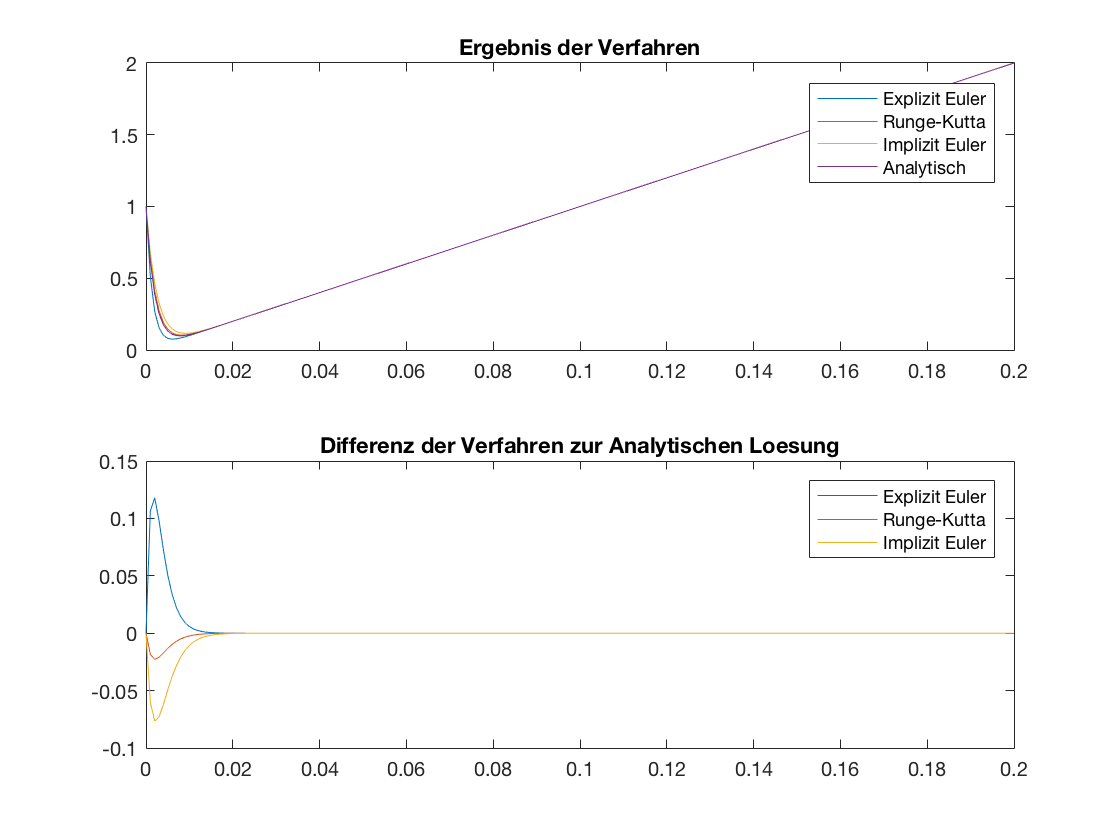
\includegraphics[width=1\linewidth]{a1_1_1}
\caption{h=0.001}
\label{fig:a1_1_1}
\end{figure}

\subsubsection{h=0.003}
Das Ergebnis zeigt, dass die Verfahren bis ca. x=0.03 unterschiedliche Ergebnisse liefern. Die Ergebnisse des Runge-Kutta-Verfahrens verlaufen bis ca. x=0.03 nahezu parallel zur analytischen Lösung. In diesem Wertebereich liefert das explizite Euler-Verfahren sehr schwankende Werte. Ab ca. x=0.03 laufen alle Kurven kongruent. Das implizite Euler Verfahren gewinnt im Gegensatz zu den anderen Verfahren durch das Steigen der Schrittweite an Genauigkeit und nähert sich in diesem Ergebnis schneller der analytischen Lösung als bei der Schrittweite von 0.001 .
\begin{figure}[H]
	\centering
	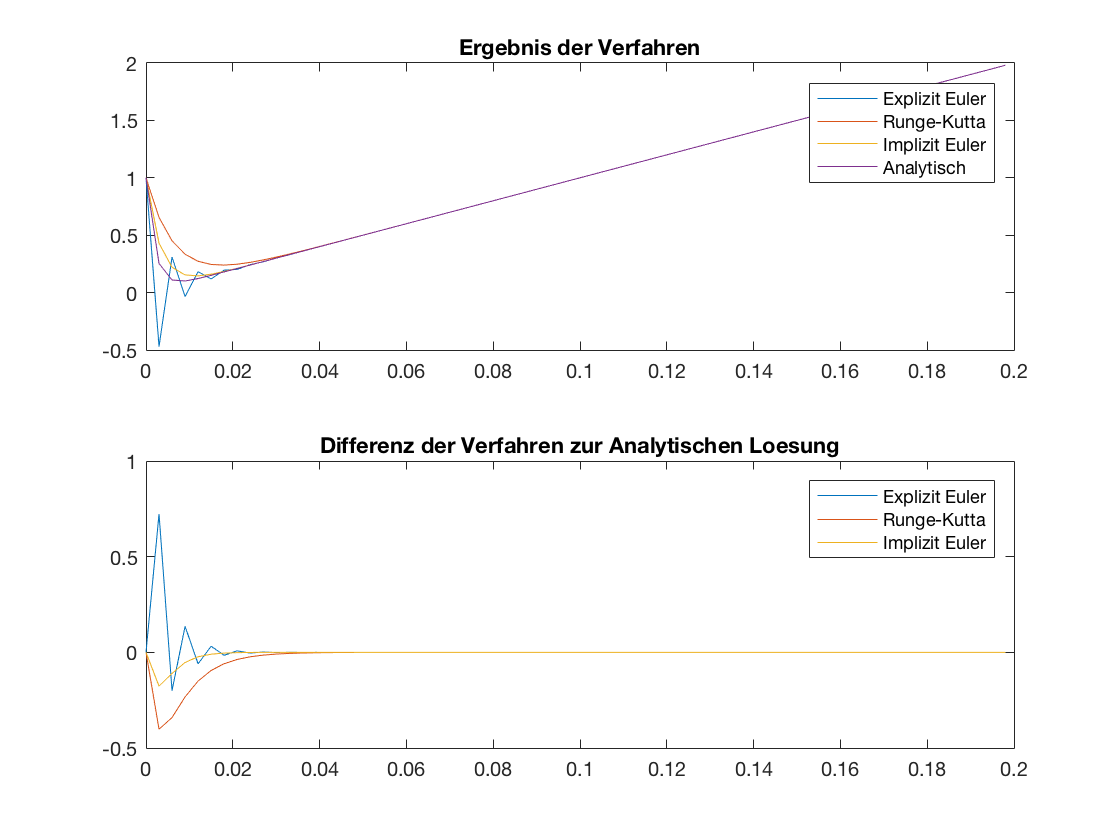
\includegraphics[width=1\linewidth]{a1_1_2}
	\caption{h=0.003}
	\label{fig:a1_1_2}
\end{figure}

\subsubsection{h=0.004}
Bis ca. x=0.01 laufen alle Kurven bis auf das des impliziten Euler Verfahrens unterschiedlich zur analytischen Lösung. Ab dort laufen die Kurven des Runge-Kutta-Verfahrens und der analytischen Lösung parallel während das implizite Euler Verfahren eine nahezu kongruente Kurve liefert. Während der ganzen Laufzeit liefert das explizite Euler-Verfahren sehr schwankende Werte, die sich mit einer Differenz von +/- 1 in der Nähe der analytischen Lösung befinden.
\begin{figure}[H]
	\centering
	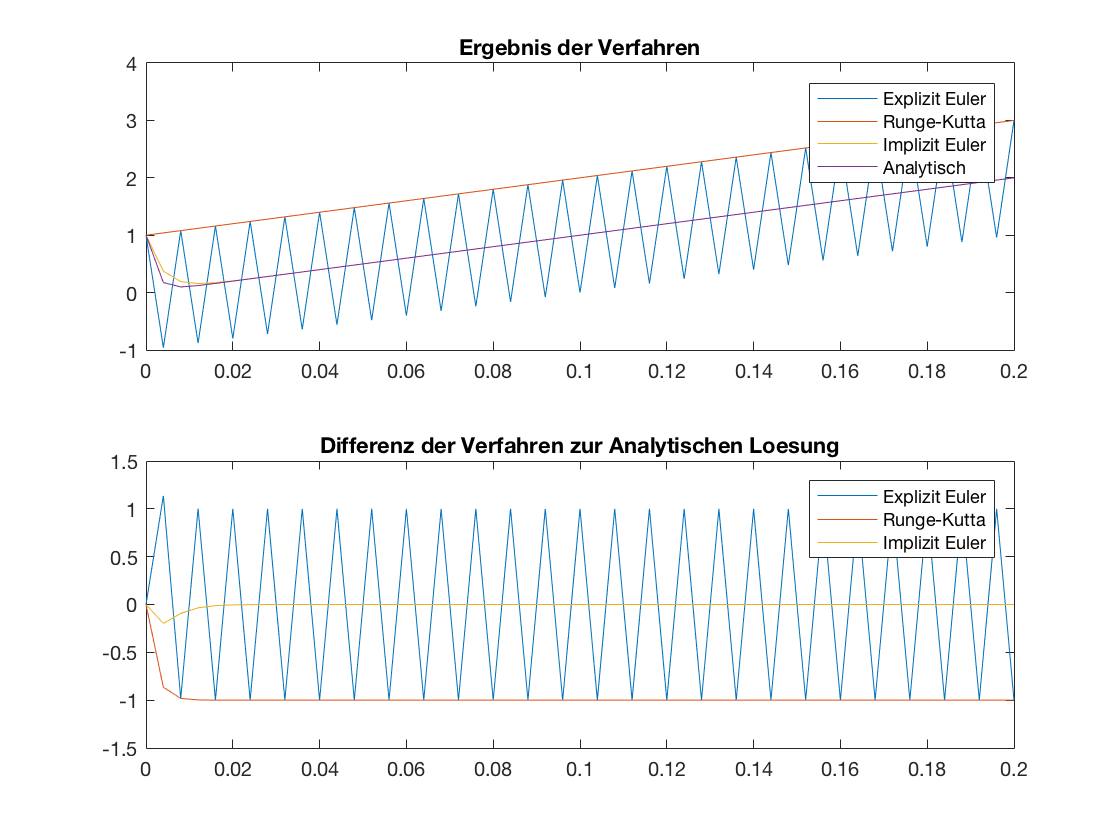
\includegraphics[width=1\linewidth]{a1_1_3}
	\caption{h=0.004}
	\label{fig:a1_1_3}
\end{figure}

\subsubsection{h=0.005}
Bis ca. x=0.15 laufen alle Kurven kongruent. Ab dort schwanken die Werte des expliziten Euler-Verfahrens mit einer Differenz von ca. +/- 0.1 um die Werte der analytischen Lösung. Die Werte des Runge-Kutta-Verfahrens hingegen werden ab ca. x=0.15 exponentiell größer und die Werte des impliziten Eulers bleiben kongruent mit der analytischen Lösung.
\begin{figure}[H]
	\centering
	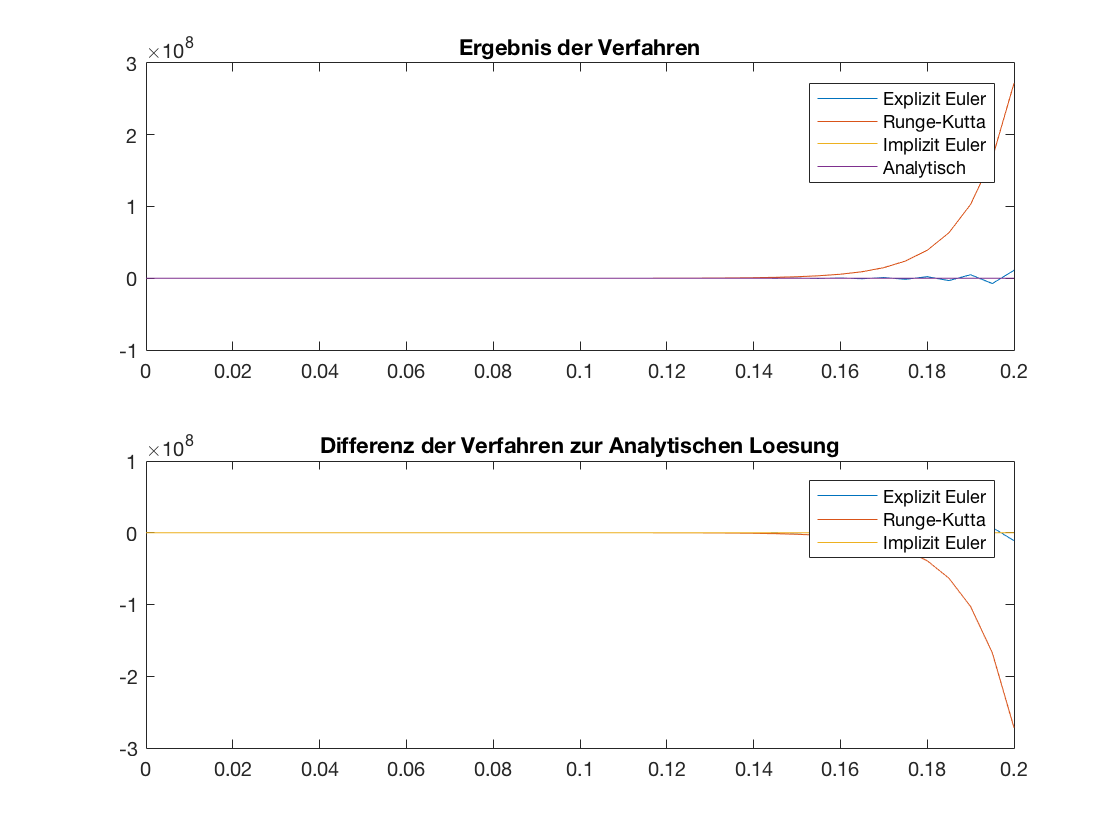
\includegraphics[width=1\linewidth]{a1_1_4}
	\caption{h=0.005}
	\label{fig:a1_1_4}
\end{figure}

\subsection{Interpretation der Ergebnisse}
Die Ergebnisse zeigen, dass die expliziten Verfahren bei einer geringen Schrittweite genauere Ergebnisse liefern. Allerdings wird dadurch die benötigte Rechenzeit erhöht. Dahingegen liefert das implizite Euler Verfahren auch bei höherer Schrittweite recht genaue Lösungen.

\section{Teilaufgabe 2 - Nicht Lineare DGL und Van der Pol}
Die folgende DGL ist gegeben: \\
$ y'' = 6 * (1 - y^{2}) * y' - y $, \\
$ y(0) = 0 $, \\
$ y'(0) = 1 $ \\



Für diese DGL ist ein Schaltbild in Simulink zu entwerfen. Des weiteren sollen die Verfahren(Runge-Kutta 2. Ordnung und expliziter Euler) erarbeitet und Iterationsgleichungen für die jeweiligen Verfahren angegeben werden, dafür muss die DGL 2. Ordnung in zwei DGLn 1. Ordnung umgewandelt werden. Im Anschluss soll ein Programm entwickelt(\textit{vanderpol}) werden das das jedes Verfahren auf die DGL anwendet und in einem Plot zum Vergleich mit der gegebenen analytischen Lösung anzeigt.\\

Das Programm (\textit{stiff}) soll mit zwei Parameter Varianten gestartet werden, die sich wie folgt beschreiben:
\begin{itemize}
	\item $h = 0.001,  t_{End} = 31 $
	\item $h = 0.02,  t_{End} = 31 $
\end{itemize}

\subsection{Schaltbild}

\begin{figure}[H]
	\centering
	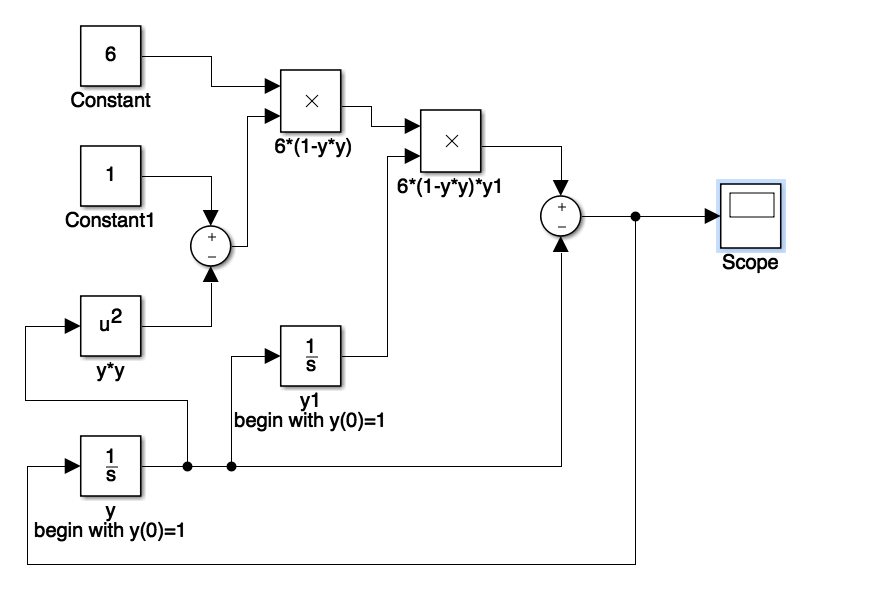
\includegraphics[width=1\linewidth]{a1_2_schaltbild}
	\caption{Simulink Schaltbild}
	\label{fig:a1_2_schaltbild}
\end{figure}

\subsection{DGLn der 1.Ordnung}
\begin{align}
\tilde{y} = y' \\
\tilde{y}' = 6 * (1 - y^{2}) * \tilde{y} - y \\
y(0)  = 0 \\
\tilde{y}(0) = 1
\end{align}

\subsection{Iterationsgleichungen}

\subsubsection{Euler-Verfahren}
\begin{align}
x_{n+1} = x_{n}+h \\
\tilde{y}_{n+1} = \tilde{y}_{n}+h*(6 * (1 - y_{n}^{2}) * \tilde{y}_{n} - y_{n}) \\
y_{n+1} = y_{n} + h * \tilde{y}_{n}
\end{align}

\subsubsection{Runge-Kutta-Verfahren 2.Ordnung}
\begin{align}
x_{n+1} = x_{n}+h \\
\tilde{k}_{1} = h * (6 * (1 - y_{n}^{2}) * \tilde{y}_{n} - y_{n}) \\
k_{1} = h * \tilde{y}_{n} \\
\tilde{k}_{2} = h * (6 * (1 - (y_{n} + \dfrac{k_{1}}{2})^{2}) * (\tilde{y}_{n} + \dfrac{\tilde{k}_{1}}{2}) - (y_{n} + \dfrac{k_{1}}{2})) \\
k_{2} = h * (\tilde{y}_{n} + \dfrac{k_{1}}{2}) \\
\tilde{y}_{n+1} = \tilde{y}_{n}+\tilde{k}_{2} \\
y_{n+1} = y_{n}+k_{2}
\end{align}

\subsection{Plot der Lösungen}
\subsubsection{h = 0.001}
\begin{figure}[H]
\centering
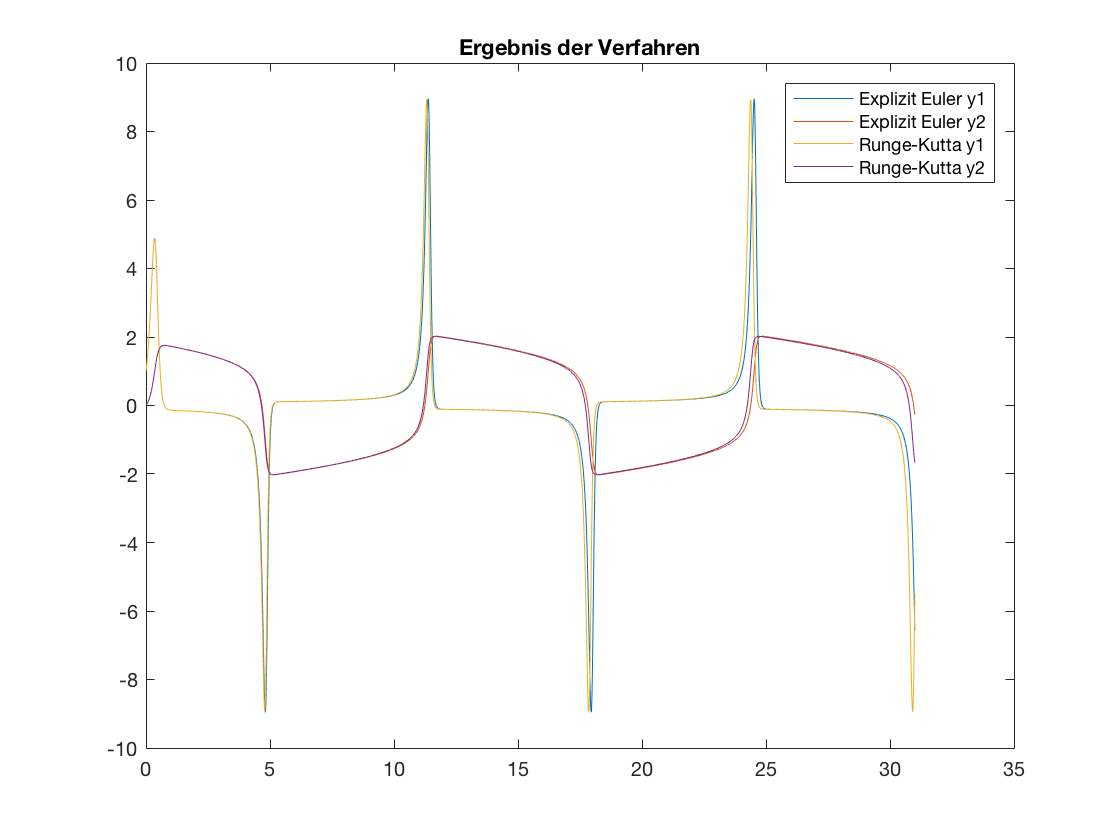
\includegraphics[width=1\linewidth]{a1_2_1}
\caption{h=0.001}
\label{fig:a1_2_1}
\end{figure}

Anhand des Ergebnisses lässt sich erkennen, dass beide Verfahren (Runge-Kutta 2.Ordnung und Expliziter Euler) bei einer Schrittweite von 0.001 kongruente Ergebnisse liefern.


\subsubsection{h = 0.02}
\begin{figure}[H]
	\centering
	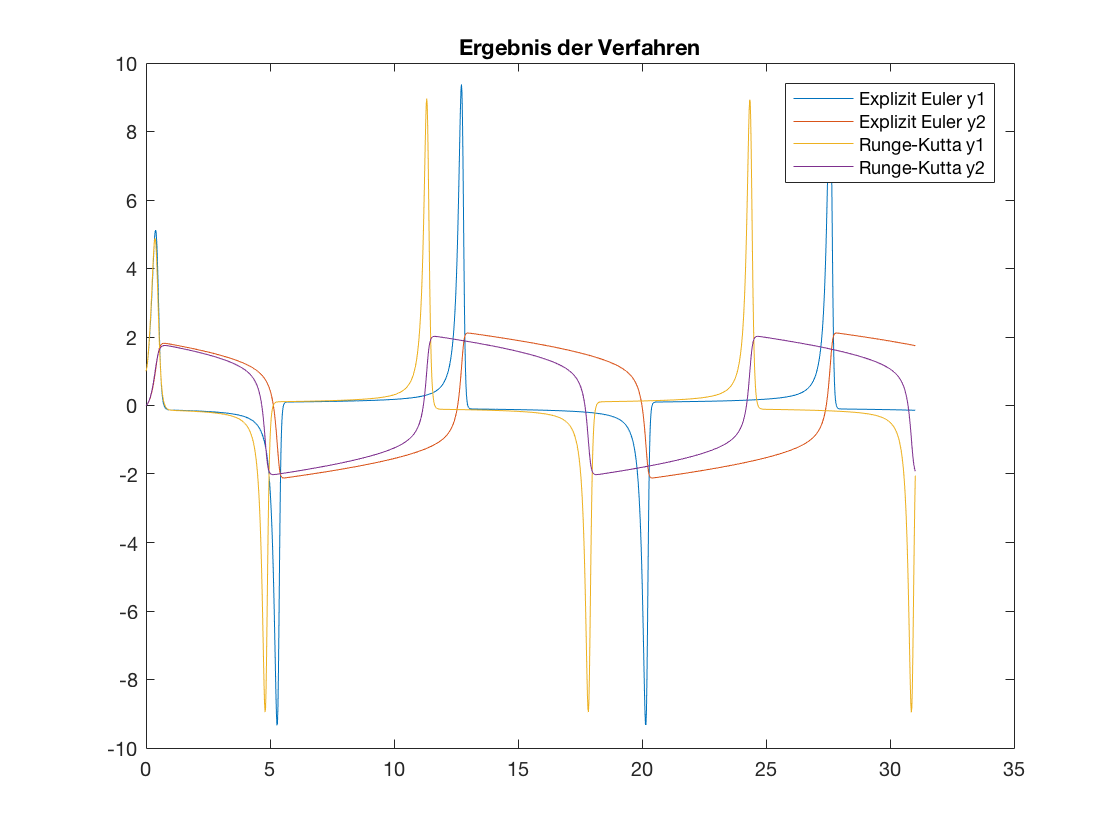
\includegraphics[width=1\linewidth]{a1_2_2}
	\caption{h=0.02}
	\label{fig:a1_2_2}
\end{figure}

In diesem Experiment mit einer Schrittweite von 0.02 verändern sich die Ergebnisse des expliziten Euler verfahrens und verschieben sich merklich gegenüber der Lösung mit einer Schrittweite von 0.001. Dahingegen verändert sich das komplexere Runge-Kutta 2. Ordnung verfahren nicht und behält das Ergebnis bei.

\section{Teilaufgabe 3 - Lorenz-Attraktor}
Es ist folgendes DGL-System gegeben: \\
$x' = -10 * (x*y)$, $x(0) = 0,01$ \\
$y' = (40 - z) * x - y$, $y(0) = 0,01$ \\
$z' = x * y - 2,67 * z$, $z(0) = 0,00$\\

Für dieses DGL System sollen die Iterationsgleichungen angegeben werden. Daraus wird ein Programm (\textit{lorenz}) entwickelt, das das DGL System löst und in zwei verschiedenen Plots sollen die Ergebnisse von $x(t)$ und von $z(t)$ dargestellt werden.
Das DGL System soll des Weiteren mit Simulink gelöst werden.\\

Das Programm soll mit folgenden Parametern gestartet werden:
\begin{itemize}
	\item $h = 0.002,  t_{End} = 120 $
\end{itemize}

Ein weiterer Vergleich soll stattfinden in dem die Funktion $y'(t)$ verändert wird. Sodass das System einmal mit $y' = (40 - z) * x - y$ und einmal mit $y' = (40.000000001 - z) * x - y$ gelöst wird. Die beiden Lösungen sollen gegenüber gestellt und verglichen werden.


\subsection{Iterationsgleichungen}
Im Folgenden die Iterationsgleichungen für das Runge-Kutta-Verfahren 2ter Ordnung bezogen auf das gegebene DGL-System.

\begin{align}
k_{1} = h * (-10 * (x_{n} * y_{n})) \\
l_{1} = h * ((40 - z) * x_{n} - y_{n}) \\
m_{1} = h * (x_{n} * y_{n} - 2,67 * z_{n}) \\
k_{2} = h*f(x_{n} + \dfrac{k_{1} }{2},y_{n} + \dfrac{l_{1} }{2},z_{n} + \dfrac{m_{1} }{2}) \\
k_{2} = h* (-10 * ((x_{n} + \dfrac{k_{1} }{2})*(y_{n} + \dfrac{l_{1} }{2})) \\
l_{2} = h*f(x_{n} + \dfrac{k_{1} }{2},y_{n} + \dfrac{l_{1} }{2},z_{n} + \dfrac{m_{1} }{2}) \\
l_{2} = h*((40 - (z_{n} + \dfrac{m_{1} }{2})) * (x_{n} + \dfrac{k_{1} }{2}) - (y_{n} + \dfrac{l_{1} }{2})) \\
m_{2} = h*f(x_{n} + \dfrac{k_{1} }{2},y_{n} + \dfrac{l_{1} }{2},z_{n} + \dfrac{m_{1} }{2}) \\
m_{2} = h*((x_{n} + \dfrac{k_{1} }{2}) * (y_{n} + \dfrac{l_{1} }{2}) - 2,67 * (z_{n} + \dfrac{m_{1} }{2})) \\
x_{n+1} = x_{n} + k2 \\
y_{n+1} = y_{n} + l2 \\
z_{n+1} = z_{n} + m2
\end{align}

\subsection{Plot der Lösung}
Gelöst durch das Runge-Kutta-Verfahren 2ter Ordnung.
\begin{figure}[H]
	\centering
	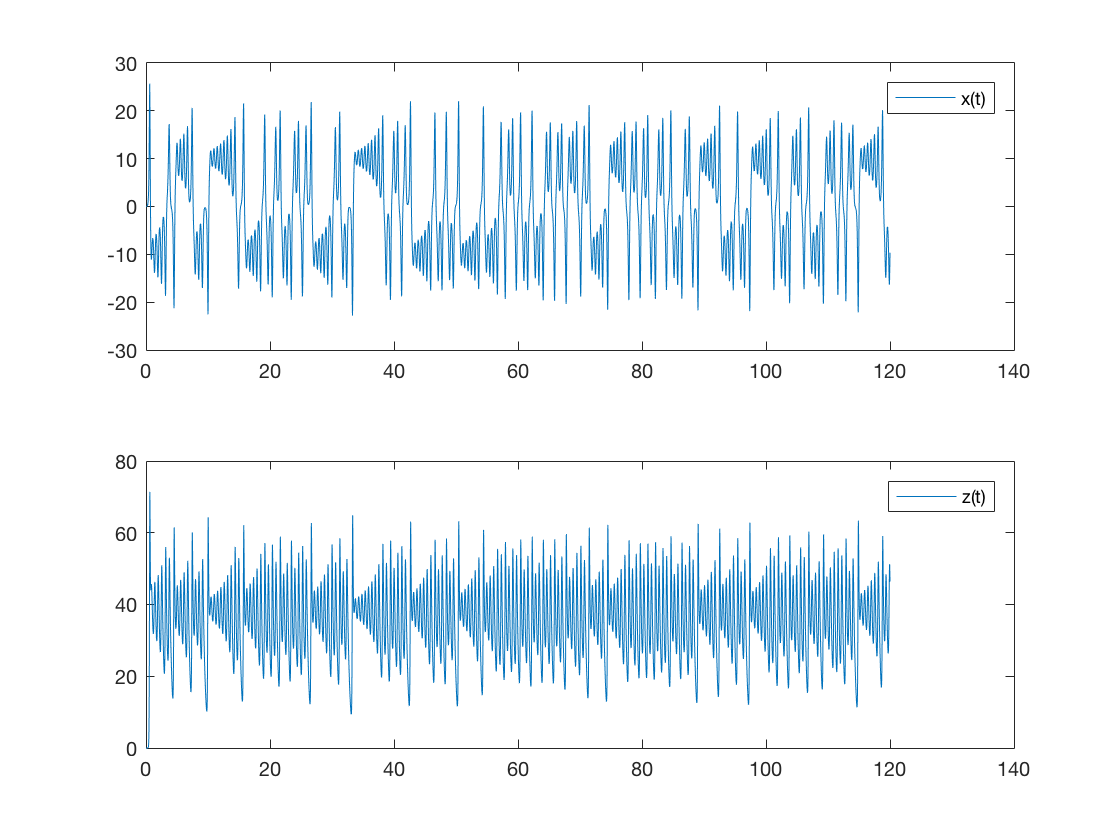
\includegraphics[width=1\linewidth]{a1_3_1}
	\caption{Vergleich von x(t) und z(t), h=0.002, $t_{end} = 120$}
	\label{fig:a1_3_1}
\end{figure}

\subsection{Schaltbild}
\begin{figure}[H]
	\centering
	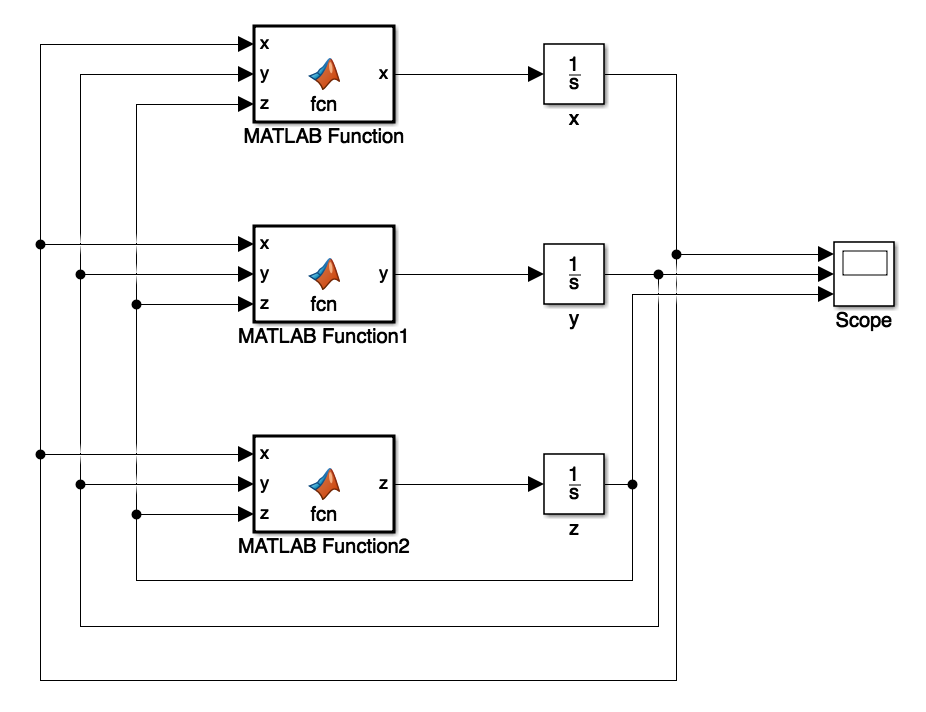
\includegraphics[width=1\linewidth]{a1_3_schaltbild}
	\caption{Simulink Schaltbild}
	\label{fig:a1_3_schaltbild}
\end{figure}

\subsection{Vergleich der Simulationen} \label{subsec:vergleich}
\begin{figure}[H]
	\centering
	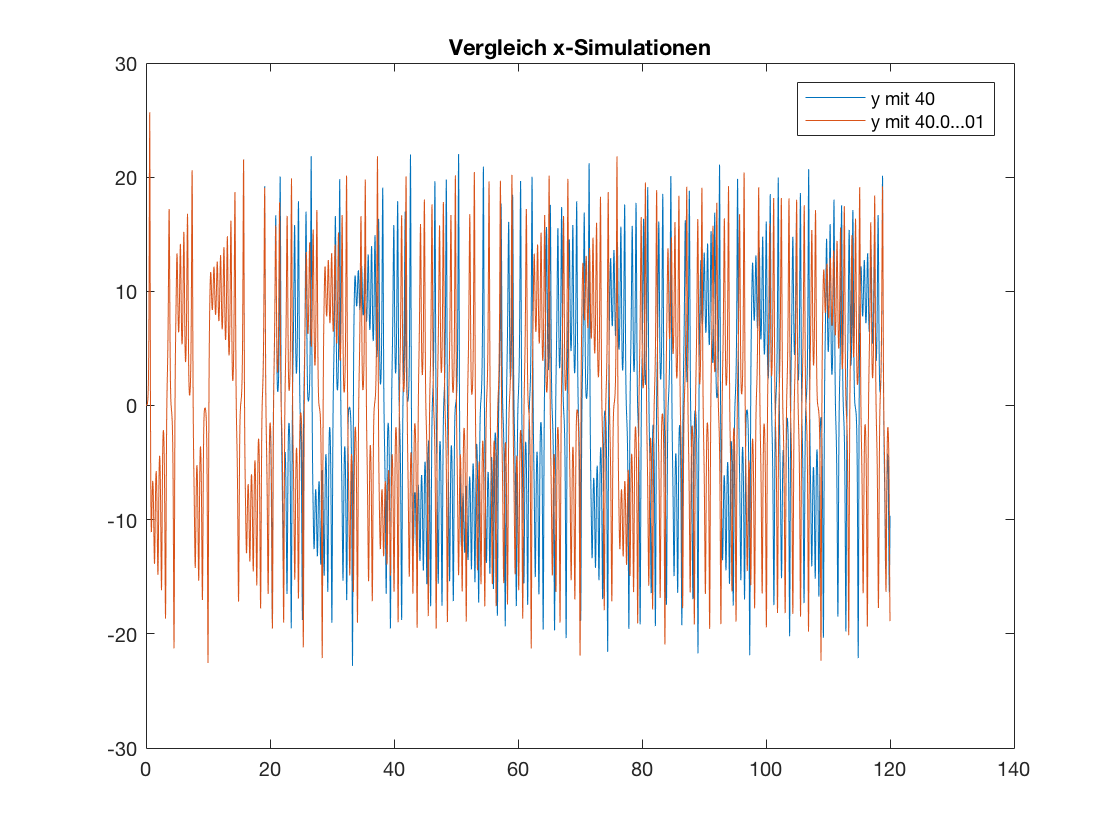
\includegraphics[width=1\linewidth]{a1_3_2}
	\caption{}
	\label{fig:a1_3_2}
\end{figure}

Durch das ausführen der zweiten Funktion y = ... mit 40.000000001 anstatt von 40 ergibt sich obenstehende Verschiebung zwischen den beiden Funktionen. Die Grafik zeigt die Lösungen des Systems mit diesem marginalen Unterschied. Da es sich bei diesem System um ein chaotisches handelt zeigt es auch die klassischen Eigenschaften eines chaotischen Systems. So sorgt eine kleine Änderung der Start Parameter für deutlich größere Änderungen im Ergebnis.

\subsection{3D Plot zum weiteren Vergleich}

Betrachtet man den 3D Plot der drei Funktionen beschreibt sich die Form des Lorenz Attraktors in diesem chaotischen Systems. Die folgende Abbildung \ref{fig:a1_3_3} veranschaulicht dieses Bild.

\begin{figure}[H]
	\centering
	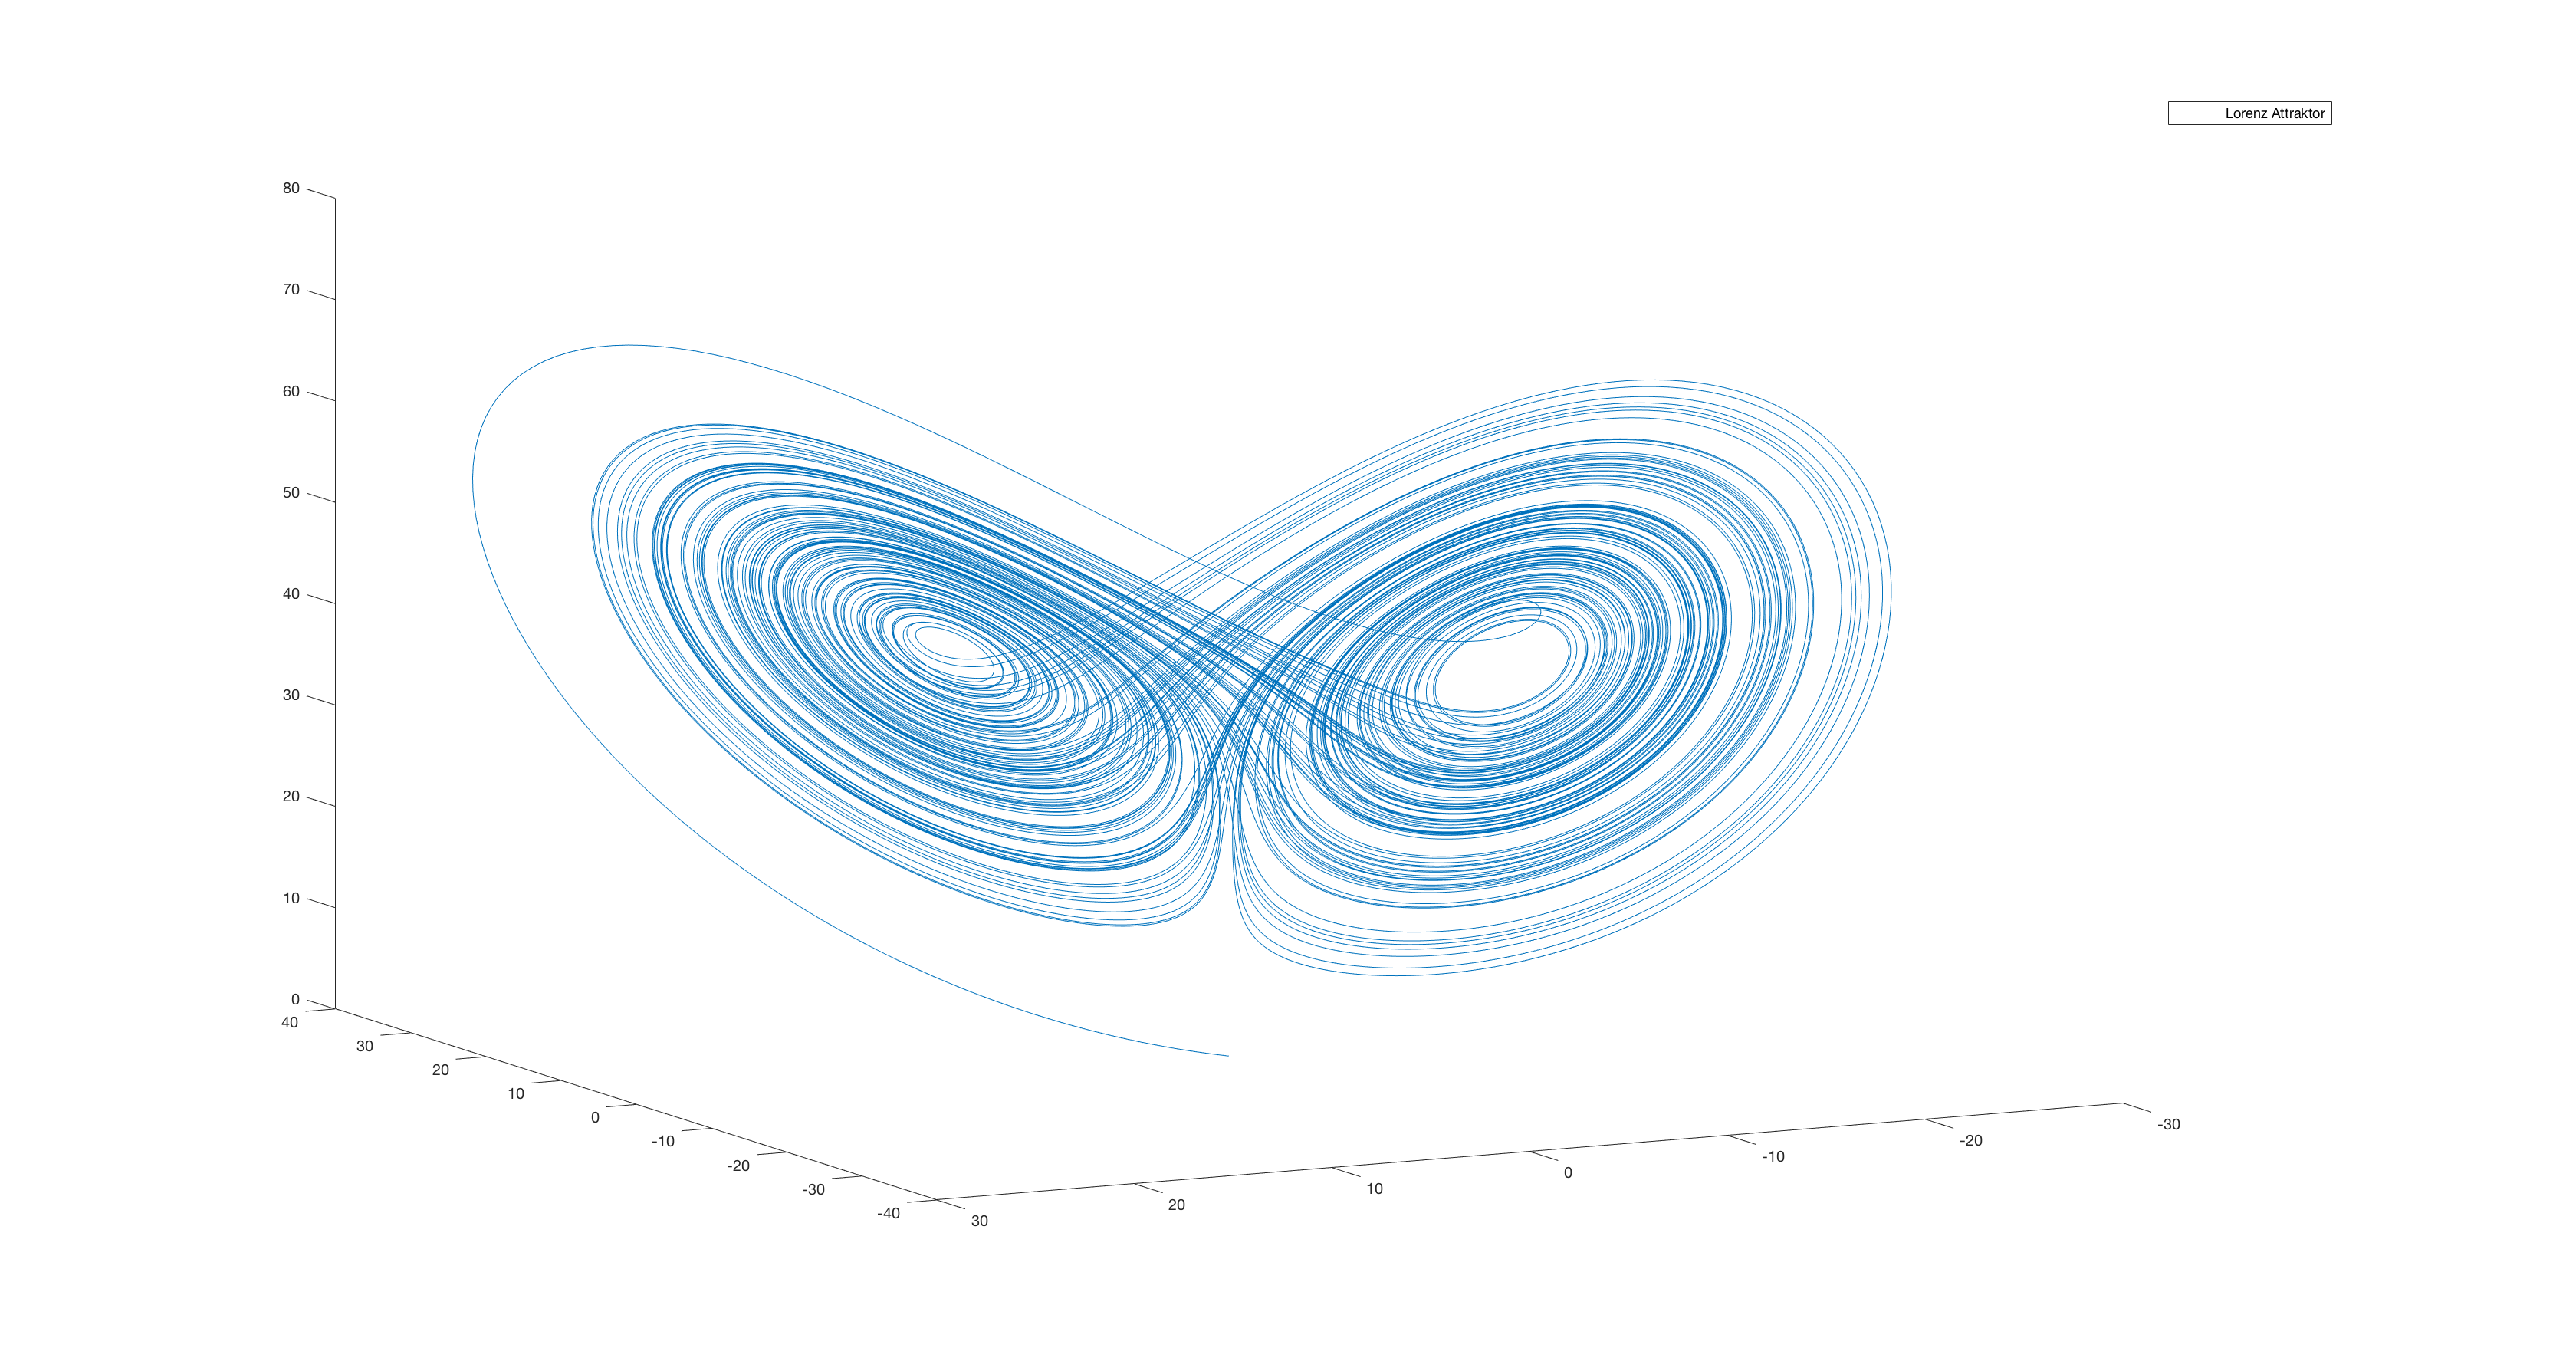
\includegraphics[width=1\linewidth]{a1_3_3}
	\caption{3D Plot des chaotischen Systems}
	\label{fig:a1_3_3}
\end{figure}

Im Vergleich dazu, die Darstellung des chaotischen Systems mit der leichten Änderung wie in Abschnitt \ref{subsec:vergleich} beschrieben siehe Abbildung \ref{fig:a1_3_4}. Hier liegen beide Systeme nebeneinander, das orange dargestellte ist das System mit der leichten Veränderung in der y-Funktion. Hier bemerkenswert ist, dass obwohl sich die Graphen in der Darstellung \ref{fig:a1_3_2} stark verschieben nehmen sie in der 3D Version in etwa den gleichen Raum ein und fügen sich recht schlüssig ineinander.

\begin{figure}[H]
	\centering
	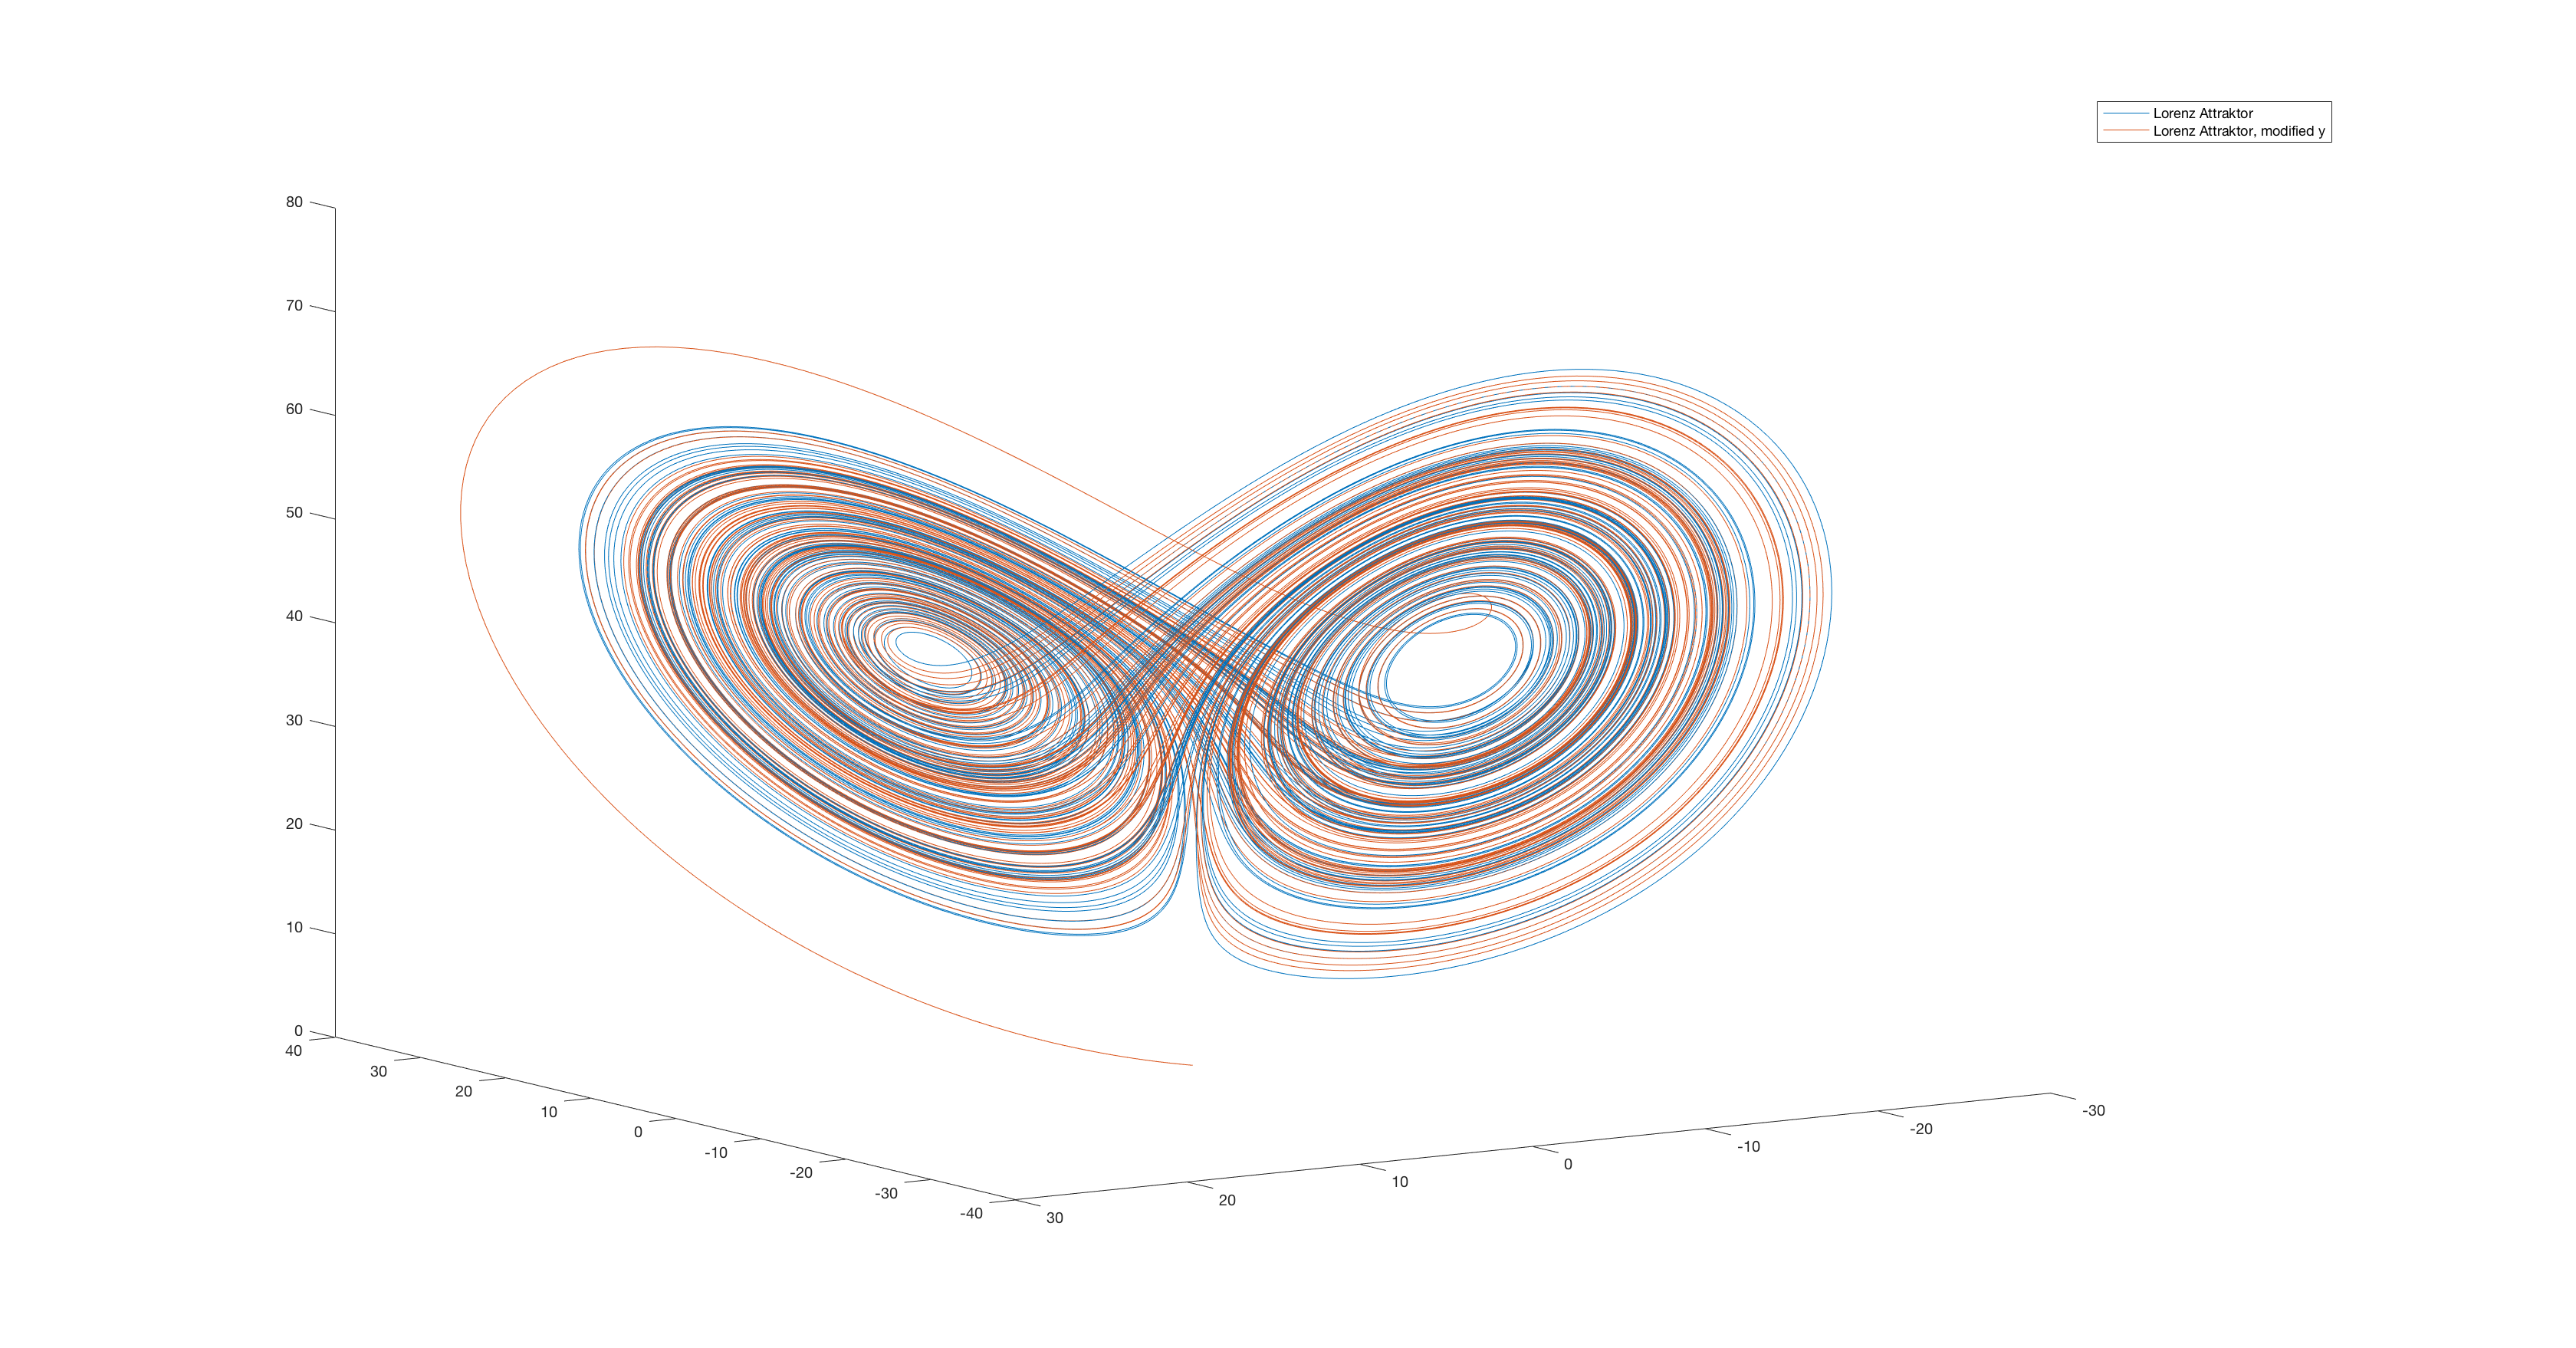
\includegraphics[width=1\linewidth]{a1_3_4}
	\caption{3D Plot der chaotischen Systeme im Vergleich}
	\label{fig:a1_3_4}
\end{figure}

\end{document}
